% Kommentare für den Editor (TexWorks/TexMakerX)
% !TeX encoding   = utf8
% !TeX spellcheck = de-DE

% --- LaTeX Vorlage ------------------------------------------------------
% speziell für einfache Dokumente wie Praktikumsprotokolle
%
% Autor: Matthias Pospiech (matthias@pospiech.eu)
% ------------------------------------------------------------------------

% Dokumentenklasse (Koma Script) -----------------------------------------
\documentclass[%
   %draft,     % Entwurfsstadium
   final,      % fertiges Dokument
   paper=a4, paper=portrait, pagesize=auto, % Papier Einstellungen
   fontsize=9pt, % Schriftgröße
   ngerman, % Sprache 
   DIV=16, % kleinere Ränder
   twocolumn, % zweispaltig
 ]{scrreprt} % Classes: scrartcl, scrreprt, scrbook
 \areaset[5mm]{0.2cm}{0.2cm}

% ~~~~~~~~~~~~~~~~~~~~~~~~~~~~~~~~~~~~~~~~~~~~~~~~~~~~~~~~~~~~~~~~~~~~~~~~
% encoding
% ~~~~~~~~~~~~~~~~~~~~~~~~~~~~~~~~~~~~~~~~~~~~~~~~~~~~~~~~~~~~~~~~~~~~~~~~

% Encoding der Dateien (sonst funktionieren Umlaute nicht)
\usepackage[utf8]{inputenc}

% Encoding der Verzeichnisse (für Pfade mit Umlauten und Leerzeichne)
\usepackage[%
   extendedchars, encoding, multidot, space,
   %filenameencoding=latin1, % Windows XP, Vista, 7
   filenameencoding=utf8,   % Linux, OS X
]{grffile}

% ~~~~~~~~~~~~~~~~~~~~~~~~~~~~~~~~~~~~~~~~~~~~~~~~~~~~~~~~~~~~~~~~~~~~~~~~
% Pakete und Stile
% ~~~~~~~~~~~~~~~~~~~~~~~~~~~~~~~~~~~~~~~~~~~~~~~~~~~~~~~~~~~~~~~~~~~~~~~~
% Schriften
% ~~~~~~~~~~~~~~~~~~~~~~~~~~~~~~~~~~~~~~~~~~~~~~~~~~~~~~~~~~~~~~~~~~~~~~~~
% Fonts Fonts Fonts
% ~~~~~~~~~~~~~~~~~~~~~~~~~~~~~~~~~~~~~~~~~~~~~~~~~~~~~~~~~~~~~~~~~~~~~~~~

% immer laden:
\usepackage[T1]{fontenc} % T1 Schrift Encoding
\usepackage{textcomp}	 % Zusätzliche Symbole (Text Companion font extension)

% ~~~~~~~~~~~~~~~~~~~~~~~~~~~~~~~~~~~~~~~~~~~~~~~~~~~~~~~~~~~~~~~~~~~~~~~~
% Symbole
% ~~~~~~~~~~~~~~~~~~~~~~~~~~~~~~~~~~~~~~~~~~~~~~~~~~~~~~~~~~~~~~~~~~~~~~~~

\usepackage{amssymb}
\usepackage{mathcomp}


%% ==== Zusammengesetzte Schriften  (Sans + Serif) =======================

%% - Latin Modern
\usepackage{lmodern}
%% -------------------

%% - Bera Schriften
%\usepackage{bera}
%% -------------------

%% - Times, Helvetica, Courier (Word Standard...)
%\usepackage{mathptmx}
%\usepackage[scaled=.90]{helvet}
%\usepackage{courier}
%% -------------------

%% - Palantino , Helvetica, Courier
%\usepackage{mathpazo}
%\usepackage[scaled=.95]{helvet}
%\usepackage{courier}
%% -------------------

%% - Charter, Bera Sans
%\usepackage{charter}\linespread{1.05}
%\renewcommand{\sfdefault}{fvs}
%\usepackage[charter]{mathdesign}



%%%% =========== Typewriter =============

%\usepackage{courier}                   %% --- Courier
%\renewcommand{\ttdefault}{cmtl}        %% --- CmBright Typewriter Font
%\usepackage[%                          %% --- Luxi Mono (Typewriter)
%   scaled=0.9
%]{luximono}



% Pakete Laden
% ~~~~~~~~~~~~~~~~~~~~~~~~~~~~~~~~~~~~~~~~~~~~~~~~~~~~~~~~~~~~~~~~~~~~~~~~
% These packages must be loaded before all others
% (primarily because they are required by other packages)
% ~~~~~~~~~~~~~~~~~~~~~~~~~~~~~~~~~~~~~~~~~~~~~~~~~~~~~~~~~~~~~~~~~~~~~~~~
\usepackage{calc}
\usepackage{fixltx2e}	% Fix known LaTeX2e bugs

\usepackage[ngerman]{babel} 	% Sprache
\usepackage[dvipsnames, table]{xcolor} 	% Farben
\usepackage[ngerman, iso]{isodate} 	%Datumsformat

% ~~~~~~~~~~~~~~~~~~~~~~~~~~~~~~~~~~~~~~~~~~~~~~~~~~~~~~~~~~~~~~~~~~~~~~~~
% Bilder, Gleitumgebungen und Platzierung
% ~~~~~~~~~~~~~~~~~~~~~~~~~~~~~~~~~~~~~~~~~~~~~~~~~~~~~~~~~~~~~~~~~~~~~~~~

\usepackage[]{graphicx}					% Graphiken
\usepackage{epstopdf}		% konvertiert eps in pdf

% provides new floats and enables H float modifier option
\usepackage{float}
% Floats immer erst nach der Referenz setzen
\usepackage{flafter}
% Alel Floats werden vor der nächsten section ausgegeben
\usepackage[section]{placeins} 
%

\usepackage{tikz}
%tikz verwenden um Grafiken zu erstellen
\usepackage{pgfplots}
%pgfplots verwenden für Diagramme

\usepackage[european, siunitx]{circuitikz}
% Schaltpläne

% ~~~~~~~~~~~~~~~~~~~~~~~~~~~~~~~~~~~~~~~~~~~~~~~~~~~~~~~~~~~~~~~~~~~~~~~~
% Beschriftungen (captions)
% ~~~~~~~~~~~~~~~~~~~~~~~~~~~~~~~~~~~~~~~~~~~~~~~~~~~~~~~~~~~~~~~~~~~~~~~~

\usepackage{caption}
\usepackage{subcaption}

% ~~~~~~~~~~~~~~~~~~~~~~~~~~~~~~~~~~~~~~~~~~~~~~~~~~~~~~~~~~~~~~~~~~~~~~~~
% Math
% ~~~~~~~~~~~~~~~~~~~~~~~~~~~~~~~~~~~~~~~~~~~~~~~~~~~~~~~~~~~~~~~~~~~~~~~~

% Base Math Package
\usepackage[fleqn]{amsmath} 
% Warnt bei Benutzung von Befehlen die mit amsmath inkompatibel sind.
\usepackage[all, error]{onlyamsmath}
%Brüche schräg statt horizontal brechen
\usepackage{nicefrac}

% ~~~~~~~~~~~~~~~~~~~~~~~~~~~~~~~~~~~~~~~~~~~~~~~~~~~~~~~~~~~~~~~~~~~~~~~~
% Science
% ~~~~~~~~~~~~~~~~~~~~~~~~~~~~~~~~~~~~~~~~~~~~~~~~~~~~~~~~~~~~~~~~~~~~~~~~

% Einheiten und Zahlenformatierung
\usepackage{siunitx}

% ~~~~~~~~~~~~~~~~~~~~~~~~~~~~~~~~~~~~~~~~~~~~~~~~~~~~~~~~~~~~~~~~~~~~~~~~
% Tables (Tabular)
% ~~~~~~~~~~~~~~~~~~~~~~~~~~~~~~~~~~~~~~~~~~~~~~~~~~~~~~~~~~~~~~~~~~~~~~~~

\usepackage{booktabs}
\usepackage{ltxtable} % Longtable + tabularx

% ~~~~~~~~~~~~~~~~~~~~~~~~~~~~~~~~~~~~~~~~~~~~~~~~~~~~~~~~~~~~~~~~~~~~~~~~
% text related packages
% ~~~~~~~~~~~~~~~~~~~~~~~~~~~~~~~~~~~~~~~~~~~~~~~~~~~~~~~~~~~~~~~~~~~~~~~~

\usepackage{url}            % Befehl \url{...}
\usepackage{enumitem}		% Kompakte Listen

% Neue Befehle: \Centering, \RaggedLeft, and \RaggedRight, ... 
\usepackage{ragged2e}


% ~~~~~~~~~~~~~~~~~~~~~~~~~~~~~~~~~~~~~~~~~~~~~~~~~~~~~~~~~~~~~~~~~~~~~~~~
% Citations
% ~~~~~~~~~~~~~~~~~~~~~~~~~~~~~~~~~~~~~~~~~~~~~~~~~~~~~~~~~~~~~~~~~~~~~~~~

%\usepackage[
%	style=alphabetic, % Loads the bibliography and the citation style 
%	natbib=true, % define natbib compatible cite commands
%]{biblatex}	
% Other options:
%	style=numeric, % 
%	style=numeric-comp,    % [1–3, 7, 8]
%	style=numeric-verb,    % [2]; [5]; [6]

\usepackage{csquotes}

% ~~~~~~~~~~~~~~~~~~~~~~~~~~~~~~~~~~~~~~~~~~~~~~~~~~~~~~~~~~~~~~~~~~~~~~~~
% layout packages
% ~~~~~~~~~~~~~~~~~~~~~~~~~~~~~~~~~~~~~~~~~~~~~~~~~~~~~~~~~~~~~~~~~~~~~~~~
%
% Befehle für 1,5 und 2 zeilig: 
% \singlespacing, \onehalfspacing und \doublespacing
\usepackage{setspace}

% ~~~~~~~~~~~~~~~~~~~~~~~~~~~~~~~~~~~~~~~~~~~~~~~~~~~~~~~~~~~~~~~~~~~~~~~~
% Kopf und Fusszeile
% ~~~~~~~~~~~~~~~~~~~~~~~~~~~~~~~~~~~~~~~~~~~~~~~~~~~~~~~~~~~~~~~~~~~~~~~~

% Kopf und Fusszeile mit scrpage2 einstellen
\usepackage[automark, komastyle, nouppercase]{scrpage2}

% ~~~~~~~~~~~~~~~~~~~~~~~~~~~~~~~~~~~~~~~~~~~~~~~~~~~~~~~~~~~~~~~~~~~~~~~~
% pdf packages
% ~~~~~~~~~~~~~~~~~~~~~~~~~~~~~~~~~~~~~~~~~~~~~~~~~~~~~~~~~~~~~~~~~~~~~~~~

% Include pages from external PDF documents in LaTeX documents
\usepackage{pdfpages} 

% Optischer Randausgleich mit pdfTeX
\usepackage{microtype}

%%% svg to tex
\newcommand{\executeiffilenewer}[3]{%
\ifnum\pdfstrcmp{\pdffilemoddate{#1}}%
{\pdffilemoddate{#2}}>0%
{\immediate\write18{#3}}\fi%
}

% Einstellungen und Layoutstile 
% ~~~~~~~~~~~~~~~~~~~~~~~~~~~~~~~~~~~~~~~~~~~~~~~~~~~~~~~~~~~~~~~~~~~~~~~~
% Colors
% ~~~~~~~~~~~~~~~~~~~~~~~~~~~~~~~~~~~~~~~~~~~~~~~~~~~~~~~~~~~~~~~~~~~~~~~~
\definecolor{sectioncolor}{RGB}{0, 0, 0}     % black

% ~~~~~~~~~~~~~~~~~~~~~~~~~~~~~~~~~~~~~~~~~~~~~~~~~~~~~~~~~~~~~~~~~~~~~~~~
% text related 
% ~~~~~~~~~~~~~~~~~~~~~~~~~~~~~~~~~~~~~~~~~~~~~~~~~~~~~~~~~~~~~~~~~~~~~~~~

%% style of URL
\urlstyle{tt}


% Keine hochgestellten Ziffern in der Fussnote (KOMA-Script-spezifisch):
\deffootnote{1.5em}{1em}{\makebox[1.5em][l]{\thefootnotemark}}

% Limit space of footnotes to 10 lines
\setlength{\dimen\footins}{10\baselineskip}

% prevent continuation of footnotes 
% at facing page
\interfootnotelinepenalty=10000 

% ~~~~~~~~~~~~~~~~~~~~~~~~~~~~~~~~~~~~~~~~~~~~~~~~~~~~~~~~~~~~~~~~~~~~~~~~
% Science
% ~~~~~~~~~~~~~~~~~~~~~~~~~~~~~~~~~~~~~~~~~~~~~~~~~~~~~~~~~~~~~~~~~~~~~~~~

\sisetup{%
	mode = math, detect-family, detect-weight,	
	exponent-product = \cdot,
	number-unit-separator=\text{\,},
	output-decimal-marker={,},
}

% ~~~~~~~~~~~~~~~~~~~~~~~~~~~~~~~~~~~~~~~~~~~~~~~~~~~~~~~~~~~~~~~~~~~~~~~~
% Citations / Style of Bibliography
% ~~~~~~~~~~~~~~~~~~~~~~~~~~~~~~~~~~~~~~~~~~~~~~~~~~~~~~~~~~~~~~~~~~~~~~~~

% Kommentar entfernene wenn biblatex geladen wird
% \IfPackageLoaded{biblatex}{%
	\ExecuteBibliographyOptions{%
%--- Backend --- --- ---
	backend=bibtex,  % (bibtex, bibtex8, biber)
	bibwarn=true, %
	bibencoding=ascii, % (ascii, inputenc, <encoding>)
%--- Sorting --- --- ---
	sorting=nty, % Sort by name, title, year.
	% other options: 
	% nty        Sort by name, title, year.
	% nyt        Sort by name, year, title.
	% nyvt       Sort by name, year, volume, title.
	% anyt       Sort by alphabetic label, name, year, title.
	% anyvt      Sort by alphabetic label, name, year, volume, title.
	% ynt        Sort by year, name, title.
	% ydnt       Sort by year (descending), name, title.
	% none       Do not sort at all. All entries are processed in citation order.
	% debug      Sort by entry key. This is intended for debugging only.
	%
	sortcase=true,
	sortlos=los, % (bib, los) The sorting order of the list of shorthands
	sortcites=false, % do/do not sort citations according to bib	
%--- Dates --- --- ---
	date=comp,  % (short, long, terse, comp, iso8601)
%	origdate=
%	eventdate=
%	urldate=
%	alldates=
	datezeros=true, %
	dateabbrev=true, %
%--- General Options --- --- ---
	maxnames=1,
	minnames=1,
%	maxbibnames=99,
%	maxcitenames=1,
%	autocite= % (plain, inline, footnote, superscript) 
	autopunct=true,
	language=auto,
	babel=none, % (none, hyphen, other, other*)
	block=none, % (none, space, par, nbpar, ragged)
	notetype=foot+end, % (foot+end, footonly, endonly)
	hyperref=true, % (true, false, auto)
	backref=true,
	backrefstyle=three, % (none, three, two, two+, three+, all+)
	backrefsetstyle=setonly, %
	indexing=false, % 
	% options:
	% true       Enable indexing globally.
	% false      Disable indexing globally.
	% cite       Enable indexing in citations only.
	% bib        Enable indexing in the bibliography only.
	refsection=none, % (part, chapter, section, subsection)
	refsegment=none, % (none, part, chapter, section, subsection)
	abbreviate=true, % (true, false)
	defernumbers=false, % 
	punctfont=false, % 
	arxiv=abs, % (ps, pdf, format)	
%--- Style Options --- --- ---	
% The following options are provided by the standard styles
	isbn=false,%
	url=false,%
	doi=false,%
	eprint=false,%	
	}%	
	
	% change alpha label to be without +	
	\renewcommand*{\labelalphaothers}{}
	
	% change 'In: <magazine>" to "<magazine>"
	\renewcommand*{\intitlepunct}{}
	\DefineBibliographyStrings{german}{in={}}
	
	% make names capitalized \textsc{}
	\renewcommand{\mkbibnamefirst}{\textsc}
	\renewcommand{\mkbibnamelast}{\textsc}
	
	% make volume and number look like 
	% 'Bd. 33(14): '
	\renewbibmacro*{volume+number+eid}{%
	  \setunit{\addcomma\space}%
	  \bibstring{volume}% 
	  \setunit{\addspace}%
	  \printfield{volume}%
	  \iffieldundef{number}{}{% 
	    \printtext[parens]{%
	      \printfield{number}%
	    }%
	  }%
	  \setunit{\addcomma\space}%
	  \printfield{eid}
	  %\setunit{\addcolon\space}%
	  }	

	% <authors>: <title>
	\renewcommand*{\labelnamepunct}{\addcolon\space}
	% make ': ' before pages
	\renewcommand*{\bibpagespunct}{\addcolon\space}
	% names delimiter ';' instead of ','
	%\renewcommand*{\multinamedelim}{\addsemicolon\space}

	% move date before issue
	\renewbibmacro*{journal+issuetitle}{%
	  \usebibmacro{journal}%
	  \setunit*{\addspace}%
	  \iffieldundef{series}
	    {}
	    {\newunit
	     \printfield{series}%
	     \setunit{\addspace}}%
	  %
	  \usebibmacro{issue+date}%
	  \setunit{\addcolon\space}%
	  \usebibmacro{issue}%
	  \setunit{\addspace}%
	  \usebibmacro{volume+number+eid}%
	  \newunit}

	% print all names, even if maxnames = 1
	\DeclareCiteCommand{\citeauthors}
	  {
	   \defcounter{maxnames}{1000}
	   \boolfalse{citetracker}%
	   \boolfalse{pagetracker}%
	   \usebibmacro{prenote}}
	  {\ifciteindex
	     {\indexnames{labelname}}
	     {}%
	   \printnames{labelname}}
	  {\multicitedelim}
	  {\usebibmacro{postnote}}

}%

% ~~~~~~~~~~~~~~~~~~~~~~~~~~~~~~~~~~~~~~~~~~~~~~~~~~~~~~~~~~~~~~~~~~~~~~~~
% figures, placement, floats and captions
% ~~~~~~~~~~~~~~~~~~~~~~~~~~~~~~~~~~~~~~~~~~~~~~~~~~~~~~~~~~~~~~~~~~~~~~~~

% Make float placement easier
\renewcommand{\floatpagefraction}{.75} % vorher: .5
\renewcommand{\textfraction}{.1}       % vorher: .2
\renewcommand{\topfraction}{.8}        % vorher: .7
\renewcommand{\bottomfraction}{.5}     % vorher: .3
\setcounter{topnumber}{3}        % vorher: 2
\setcounter{bottomnumber}{2}     % vorher: 1
\setcounter{totalnumber}{5}      % vorher: 3

%% ~~~ Captions ~~~~~~~~~~~~~~~~~~~~~~~~~~~~~~~~~~~~~~~~~~~~~~~~~~~~~~~~~~
% Style of captions
\DeclareCaptionStyle{captionStyleTemplateDefault}
[ % single line captions
   justification = centering
]
{ % multiline captions
% -- Formatting
   format      = plain,  % plain, hang
   indention   = 0em,    % indention of text 
   labelformat = default,% default, empty, simple, brace, parens
   labelsep    = colon,  % none, colon, period, space, quad, newline, endash
   textformat  = simple, % simple, period
% -- Justification
   justification = justified, %RaggedRight, justified, centering
   singlelinecheck = true, % false (true=ignore justification setting in single line)
% -- Fonts
   labelfont   = {small,bf},
   textfont    = {small,rm},
% valid values:
% scriptsize, footnotesize, small, normalsize, large, Large
% normalfont, ip, it, sl, sc, md, bf, rm, sf, tt
% singlespacing, onehalfspacing, doublespacing
% normalcolor, color=<...>
%
% -- Margins and further paragraph options
   margin = 10pt, %.1\textwidth,
   % width=.8\linewidth,
% -- Skips
   skip     = 10pt, % vertical space between the caption and the figure
   position = auto, % top, auto, bottom
% -- Lists
   % list=no, % suppress any entry to list of figure 
   listformat = subsimple, % empty, simple, parens, subsimple, subparens
% -- Names & Numbering
   % figurename = Abb. %
   % tablename  = Tab. %
   % listfigurename=
   % listtablename=
   % figurewithin=chapter
   % tablewithin=chapter
%-- hyperref related options
	hypcap=true, % (true, false) 
	% true=all hyperlink anchors are placed at the 
	% beginning of the (floating) environment
	%
	hypcapspace=0.5\baselineskip
}

% apply caption style
\captionsetup{
	style = captionStyleTemplateDefault % base
}

% Predefinded skip setup for different floats
\captionsetup[table]{position=top}
\captionsetup[figure]{position=bottom}


% options for subcaptions
\captionsetup[sub]{ %
	style = captionStyleTemplateDefault, % base
	skip=6pt,
	margin=5pt,
	labelformat = parens,% default, empty, simple, brace
	labelsep    = space,
	list=false,
	hypcap=false
}

% ~~~~~~~~~~~~~~~~~~~~~~~~~~~~~~~~~~~~~~~~~~~~~~~~~~~~~~~~~~~~~~~~~~~~~~~~
% layout 
% ~~~~~~~~~~~~~~~~~~~~~~~~~~~~~~~~~~~~~~~~~~~~~~~~~~~~~~~~~~~~~~~~~~~~~~~~


%% Paragraph Separation =================================
\KOMAoptions{%
   parskip=absolute, % do not change indentation according to fontsize
   parskip=false     % indentation of 1em
   % parskip=half    % parksip of 1/2 line 
}%

%% line spacing =========================================
%\onehalfspacing	% 1,5-facher Abstand
%\doublespacing		% 2-facher Abstand

%% page layout ==========================================

\raggedbottom     % Variable Seitenhoehen zulassen

% Koma Script text area layout
\KOMAoptions{%
   DIV=11,% (Size of Text Body, higher values = greater textbody)
   BCOR=5mm% (Bindekorrektur)
}%

%%% === Page Layout  Options ===
\KOMAoptions{% (most options are for package typearea)
   % twoside=true, % two side layout (alternating margins, standard in books)
   twoside=false, % single side layout 
   %
   headlines=2.1,%
}%

%\KOMAoptions{%
%      headings=noappendixprefix % chapter in appendix as in body text
%      ,headings=nochapterprefix  % no prefix at chapters
%      % ,headings=appendixprefix   % inverse of 'noappendixprefix'
%      % ,headings=chapterprefix    % inverse of 'nochapterprefix'
%      % ,headings=openany   % Chapters start at any side
%      % ,headings=openleft  % Chapters start at left side
%      ,headings=openright % Chapters start at right side      
%}%


% reloading of typearea, necessary if setting of spacing changed
\typearea[current]{last}

%% Zitate
\renewcommand*{\dictumwidth}{0.5\textwidth}

% ~~~~~~~~~~~~~~~~~~~~~~~~~~~~~~~~~~~~~~~~~~~~~~~~~~~~~~~~~~~~~~~~~~~~~~~~
% Titlepage
% ~~~~~~~~~~~~~~~~~~~~~~~~~~~~~~~~~~~~~~~~~~~~~~~~~~~~~~~~~~~~~~~~~~~~~~~~
\KOMAoptions{%
   % titlepage=true %
   titlepage=false %
}%

% ~~~~~~~~~~~~~~~~~~~~~~~~~~~~~~~~~~~~~~~~~~~~~~~~~~~~~~~~~~~~~~~~~~~~~~~~
% head and foot lines
% ~~~~~~~~~~~~~~~~~~~~~~~~~~~~~~~~~~~~~~~~~~~~~~~~~~~~~~~~~~~~~~~~~~~~~~~~

% \pagestyle{scrheadings} % Seite mit Headern
\pagestyle{scrplain} % Seiten ohne Header

% loescht voreingestellte Stile
\clearscrheadings
\clearscrplain
%
% Was steht wo...
% Bei headings:
%   % Oben aussen: Kapitel und Section
%   % Unten aussen: Seitenzahl
%   \ohead{\pagemark}
%   \ihead{\headmark}
%   \ofoot[\pagemark]{} % Außen unten: Seitenzahlen bei plain
% Bei Plain:
\cfoot[\pagemark]{\pagemark} % Mitte unten: Seitenzahlen bei plain


% Angezeigte Abschnitte im Header
% \automark[section]{chapter} %[rechts]{links}
\automark[subsection]{section} %[rechts]{links}

% ~~~~~~~~~~~~~~~~~~~~~~~~~~~~~~~~~~~~~~~~~~~~~~~~~~~~~~~~~~~~~~~~~~~~~~~~
% headings / page opening
% ~~~~~~~~~~~~~~~~~~~~~~~~~~~~~~~~~~~~~~~~~~~~~~~~~~~~~~~~~~~~~~~~~~~~~~~~
\setcounter{secnumdepth}{3}

\KOMAoptions{%
%%%% headings
   % headings=small  % Small Font Size, thin spacing above and below
   % headings=normal % Medium Font Size, medium spacing above and below
   headings=big % Big Font Size, large spacing above and below
}%

% Titelzeile linksbuendig, haengend
\renewcommand*{\raggedsection}{\raggedright} 

% ~~~~~~~~~~~~~~~~~~~~~~~~~~~~~~~~~~~~~~~~~~~~~~~~~~~~~~~~~~~~~~~~~~~~~~~~
% fonts of headings
% ~~~~~~~~~~~~~~~~~~~~~~~~~~~~~~~~~~~~~~~~~~~~~~~~~~~~~~~~~~~~~~~~~~~~~~~~
\setkomafont{sectioning}{\normalfont\sffamily} % \rmfamily
\setkomafont{descriptionlabel}{\itshape}
\setkomafont{pageheadfoot}{\normalfont\normalcolor\small\sffamily}
\setkomafont{pagenumber}{\normalfont\sffamily}

%%% --- Titlepage ---
%\setkomafont{subject}{}
%\setkomafont{subtitle}{}
%\setkomafont{title}{}

% ~~~~~~~~~~~~~~~~~~~~~~~~~~~~~~~~~~~~~~~~~~~~~~~~~~~~~~~~~~~~~~~~~~~~~~~~
% settings and layout of TOC, LOF, 
% ~~~~~~~~~~~~~~~~~~~~~~~~~~~~~~~~~~~~~~~~~~~~~~~~~~~~~~~~~~~~~~~~~~~~~~~~
\setcounter{tocdepth}{3} % Depth of TOC Display

% ~~~~~~~~~~~~~~~~~~~~~~~~~~~~~~~~~~~~~~~~~~~~~~~~~~~~~~~~~~~~~~~~~~~~~~~~
% Tabellen
% ~~~~~~~~~~~~~~~~~~~~~~~~~~~~~~~~~~~~~~~~~~~~~~~~~~~~~~~~~~~~~~~~~~~~~~~~

%%% -| Neue Spaltendefinitionen 'columntypes' |--
%
% Belegte Spaltentypen:
% l - links
% c - zentriert
% r - rechts
% p,m,b  - oben, mittig, unten
% X - tabularx Auto-Spalte

% um Tabellenspalten mit Flattersatz zu setzen, muss \\ vor
% (z.B.) \raggedright geschuetzt werden:
\newcommand{\PreserveBackslash}[1]{\let\temp=\\#1\let\\=\temp}

% Spalten mit Flattersatz und definierte Breite:
% m{} -> mittig
% p{} -> oben
% b{} -> unten
%
% Linksbuendig:
\newcolumntype{v}[1]{>{\PreserveBackslash\RaggedRight\hspace{0pt}}p{#1}}
\newcolumntype{M}[1]{>{\PreserveBackslash\RaggedRight\hspace{0pt}}m{#1}}
% % Rechtsbuendig :
% \newcolumntype{R}[1]{>{\PreserveBackslash\RaggedLeft\hspace{0pt}}m{#1}}
% \newcolumntype{S}[1]{>{\PreserveBackslash\RaggedLeft\hspace{0pt}}p{#1}}
% % Zentriert :
% \newcolumntype{Z}[1]{>{\PreserveBackslash\Centering\hspace{0pt}}m{#1}}
% \newcolumntype{A}[1]{>{\PreserveBackslash\Centering\hspace{0pt}}p{#1}}

\newcolumntype{Y}{>{\PreserveBackslash\RaggedLeft\hspace{0pt}}X}

%-- Einstellungen für Tabellen ----------
\providecommand\tablestyle{%
  \renewcommand{\arraystretch}{1.4} % Groessere Abstaende zwischen Zeilen
  \normalfont\normalsize            %
  \sffamily\small           % Serifenlose und kleine Schrift
  \centering%                       % Tabelle zentrieren
}

%--Einstellungen für Tabellen ----------

\colorlet{tablesubheadcolor}{gray!40}
\colorlet{tableheadcolor}{gray!25}
\colorlet{tableblackheadcolor}{black!60}
\colorlet{tablerowcolor}{gray!15.0}


% ~~~~~~~~~~~~~~~~~~~~~~~~~~~~~~~~~~~~~~~~~~~~~~~~~~~~~~~~~~~~~~~~~~~~~~~~
% pdf packages
% ~~~~~~~~~~~~~~~~~~~~~~~~~~~~~~~~~~~~~~~~~~~~~~~~~~~~~~~~~~~~~~~~~~~~~~~~

% ~~~~~~~~~~~~~~~~~~~~~~~~~~~~~~~~~~~~~~~~~~~~~~~~~~~~~~~~~~~~~~~~~~~~~~~~
% fix remaining problems
% ~~~~~~~~~~~~~~~~~~~~~~~~~~~~~~~~~~~~~~~~~~~~~~~~~~~~~~~~~~~~~~~~~~~~~~~~




% ~~~~~~~~~~~~~~~~~~~~~~~~~~~~~~~~~~~~~~~~~~~~~~~~~~~~~~~~~~~~~~~~~~~~~~~~
% Eigene Befehle
% ~~~~~~~~~~~~~~~~~~~~~~~~~~~~~~~~~~~~~~~~~~~~~~~~~~~~~~~~~~~~~~~~~~~~~~~~
% -- new commands --
\providecommand{\abs}[1]{\lvert#1\rvert}
\providecommand{\Abs}[1]{\left\lvert#1\right\rvert}
\providecommand{\norm}[1]{\left\Vert#1\right\Vert}
\providecommand{\Trace}[1]{\ensuremath{\Tr\{\,#1\,\}}} % Trace /Spur
%

\renewcommand{\d}{\partial\mspace{2mu}} % partial diff
\newcommand{\td}{\,\mathrm{d}}	% total diff

\newcommand{\Ham}{\mathcal{H}}    % Hamilton
\newcommand{\Prob}{\mathscr{P}}    % Hamilton
\newcommand{\unity}{\mathds{1}}   % Real

\renewcommand{\i}{\mathrm{i}}   % imagin�re Einheit



% -- New Operators --
\DeclareMathOperator{\rot}{rot}
\DeclareMathOperator{\grad}{grad}
\DeclareMathOperator{\Tr}{Tr}
\DeclareMathOperator{\const}{const}
\DeclareMathOperator{\e}{e} 			% exponatial Function


%\renewcommand{\labelenumi}{\alph{enumi})}
%\renewcommand{\labelenumii}{\roman{enumii})}
\setlength{\parindent}{0pt}
% ~~~~~~~~~~~~~~~~~~~~~~~~~~~~~~~~~~~~~~~~~~~~~~~~~~~~~~~~~~~~~~~~~~~~~~~~
% Eigene Befehle
% ~~~~~~~~~~~~~~~~~~~~~~~~~~~~~~~~~~~~~~~~~~~~~~~~~~~~~~~~~~~~~~~~~~~~~~~~
% Silbentrennung hinzufügen als 
% Sil-ben-tren-nung 
\hyphenation{}

\listfiles % schreibt alle verwendeten Dateien in die log Datei

%% Dokument Beginn %%%%%%%%%%%%%%%%%%%%%%%%%%%%%%%%%%%%%%%%%%%%%%%%%%%%%%%%
\begin{document}
%\includepdf{content/Deckblatt_WI}
%% Automatische Titelseite

\subject{Elektronik}
\title{Formelsammlung\\}
\author{\includegraphics[width=6.5cm]{images/logo}\\ \\  David Mändlen \& Benjamin Braun}
\date{\today}
\maketitle

% Manuelle Titelseite

%\begin{titlepage}
%   \mbox{}\vspace{5\baselineskip}\\
%   \sffamily\huge
%   \centering
%   % Titel
%   \LaTeXe{}-Vorlage von Matthias Pospiech
%   \vspace{3\baselineskip}\\
%   \rmfamily\Large
%   Leibniz Universität Hannover
%   \vspace{2\baselineskip}\\
%   \rmfamily\Large
%   Matthias Pospiech
%   \vspace{1\baselineskip}\\
%   \today
%\end{titlepage}


%\clearpage

\null

\vfill

\dictum[Dr. Axel Stoll]{Magie ist Physik durch Wollen!}

\clearpage

%\tableofcontents

% Testdokumente (auskommentieren!)
%\input{content/demo/demo.tex}
%\input{content/demo/latexexample.tex}

% in diese Datei gehört der Inhalt des Dokumentes:
%\input{content/Fehlerrechnung.tex}
%\input{content/Vorbereitung.tex}
\documentclass[a4paper, 8pt, twocolumn]{scrreprt}
\usepackage[top=8pt, left=8pt, right=8pt, bottom=8pt]{geometry}
\usepackage{graphicx}
\usepackage[export]{adjustbox}
\usepackage[ngerman]{babel}
\usepackage[utf8]{inputenc}
\begin{document}
\chapter{Objektorientiertes Design}\label{objektorientiertes-design}

\section{SOLID}\label{solid}

\paragraph{Single Responsibility}\label{single-responsibility}

Jede Klasse sollte nur eine Verantwortung haben (Unix-Philosophie)

Grund: steigende Änderungswahrscheinlichkeit führt zu steigender
Fehlerwahrscheinlichkeit

\paragraph{Open-Closed-Prinzip}\label{open-closed-prinzip}

Klassen sollten für Erweiterungen offen sein, gleichzeitig aber ihr
Verhalten nicht ändern. (open for extension, closed for modification)

Beispiel: Vererbung ändert Basisverhalten nicht, erweitert aber um
zusätzliche Funktionen oder Daten.

\paragraph{Liskovsches
stitutionsprinzip}\label{liskovsches-substitutionsprinzip}

Instanzen von abgeleiteten Klassen müssen sich so verhalten, dass sie
das Verhalten der Basisklasse 1:1 abbilden können. Überschriebene
Methoden dürfen ihr Basisverhalten nicht ändern.

Ziel: Vermeidung von Überraschungen beim Anwender.

\paragraph{Interface Segregation}\label{interface-segregation}

Clients sollten nicht dazu gezwungen werden, von Interfaces abzuhängen,
die sie nicht verwenden. Clients agieren nur mit Interfaces, die das und
\emph{nur} das implementieren, was die Clients benötigen.

Ziel: Aufteilung großer Interfaces und Reduktion unnötiger
Abhängigkeiten.

\paragraph{Dependency Inversion}\label{dependency-inversion}

Abhängigkeiten sollten von kronkreteren Modulen niedrigerer Ebenen zu
abstrakten Modulen höherer Ebenen gerichtet sein.

Ziel: Reduktion von Abhängigkeiten zwischen Modulen.

\paragraph{Dependency Lookup}\label{dependency-lookup}

Objekt sucht nach benötigtem Objekt, beispielsweise in einem Register.
Damit hängt es nicht von jedem benötigten Objekt ab, sondern nur vom
Register. Das Objekt stellt zur Laufzeit seine Verknüpfung mit einem
anderen Objekt her, indem es nach einem logischen Namen sucht. (Aktiv)

Beispiel: Person ruft Escort-Service an und fragt gezielt nach
``Scarlett O'Hara''.

\paragraph{Dependency Injection}\label{dependency-injection}

Erzeugung von Objekten und Zuordnungen von Abhängigkeiten werden an eine
dritte Partei delegiert, damit sind die Objekte voneinander nicht
abhängig. Abhängigkeiten werden von außen injiziert. (Passiv)

Beispiel: Der Escort-Service weiß, was seine Kunden brauchen und teilt
diesen ohne Nachfragen oder Auftrag eine Escort-Dame zu.

\section{Kopplung}\label{kopplung}

\paragraph{Strong cohesion}\label{strong-cohesion}

Eine Klasse mit ``strong cohesion'' hat wenige, wohldefinierte Aufgaben,
die eng miteinander verwandt sind.

Beispiel: High Cohesion: Escort-Dame. Low Cohesion: Partnerin.

\paragraph{Loose coupling}\label{loose-coupling}

Komponenten einer Software kommunizieren nur über wenige Schnittstellen
mit anderen Komponenten, dadurch ist die Abhängigkeit sehr gering.
Globale Variablen, öffentliche Attribute, Singletons, Zustände in
Datenbanken: Schlecht, da sie Schnittstellen vergrößern.

\begin{figure} [h]
	\raggedright
	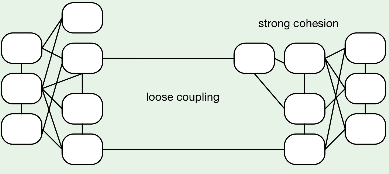
\includegraphics[width=0.3\textwidth]{images/loose_coupling}
\end{figure}

{\let\clearpage\relax \chapter{Architekturmuster}\label{architekturmuster}}

\section{Unterschied Architektur- zu
Entwurfsmuster}\label{unterschied-architektur--zu-entwurfsmuster}

Architekturmuster beziehen sich auf das Gesamtsystem (grundlegendes
Problem), während sich Entwurfsmuster auf die Teilgebiete und die
Umsetzung beziehen (lokales Problem)

Beispiel: Einkommensgenerierung. Architektur: Gründung Escort-Service.
Entwurf: Standort, Personal, Verwaltung.

\section{Layer}\label{layer}

Software ist in logischen Schichten organisiert. Problem:

\begin{itemize}
\itemsep1pt\parskip0pt\parsep0pt
\item
  Unterteilung komplexer Systeme (Abhängigkeitsminimierung)
\item
  Horizontale Strukturierung (Obere Schicht = Client, Untere Schicht =
  Server)
\item
  Jede Schicht repräsentiert eine Abstraktion
\end{itemize}

Lösung:

\begin{itemize}
\itemsep1pt\parskip0pt\parsep0pt
\item
  Jede Schicht verfolgt einen bestimmten Zweck
\item
  Client-Server Modell
\end{itemize}

\paragraph{strict layering / closed
architecture}\label{strict-layering-closed-architecture}

Schichten dürfen nicht übersprungen werden und dürfen nur die direkt
darunter liegende Schicht aufrufen.

Vorteil: leichter test- und wartbar.

\paragraph{loose layering / open
architecture}\label{loose-layering-open-architecture}

Schichten dürfen übersprungen werden, höchste Schicht kann direkt mit
tiefster Schicht kommunizieren.

Vorteil: höhere Performanz.

\section{Pipes and Filters}\label{pipes-and-filters}

Filter modifizieren Daten, Pipes transportieren Daten. Problem:

\begin{itemize}
\itemsep1pt\parskip0pt\parsep0pt
\item
  Unterteilung Datenstrom in Einzelschritte
\item
  Einfach erweiterbar
\item
  Parallelverarbeitung gut möglich
\end{itemize}

Lösung:

\begin{itemize}
\itemsep1pt\parskip0pt\parsep0pt
\item
  Zerlegung in Einzelschritte
\item
  Jeder Verarbeitungsschritt ist ein Filter
\item
  Jeder Transportweg ist eine Pipe
\item
  Filter lesen, verarbeiten und geben Daten aus
\item
  Pipes transportieren und puffern Daten
\item
  Pipes entkoppeln Entitäten
\item
  Asynchrone Schreib- und Lesevorgänge möglich
\end{itemize}

\paragraph{Aktiver Filter}\label{aktiver-filter}

Eigenständig laufende Prozesse oder Threads, werden nach Instanziierung
von übergeordnetem Programmteil aufgerufen. Laufen kontinuierlich.

\paragraph{Passiver Filter}\label{passiver-filter}

Aufruf durch benachbartes Filterelement.

\paragraph{Push}\label{push}

Vorgänger hat Ausgabedaten erzeugt und ruft zu aktivierenden Filter auf.
(Daten werden zur Verfügung gestellt)

\paragraph{Pull}\label{pull}

Nachfolger fordert Daten an. (Daten werden benötigt)

\section{Plug-In}\label{plug-in}

Interface beschreibt Funktion, Plug-Ins sind die konkreten Umsetzungen
dieser Interfaces. Der \textbf{Plugin-Manager} sorgt für die korrekte Zuordnung
der konkreten Umsetzung zum Interface bei Aufruf.

Problem:

\begin{itemize}
\itemsep1pt\parskip0pt\parsep0pt
\item
  Erweiterbarkeit ohne Modifikation
\item
  Neue Funktionalität durch Dritte
\item
  Core-System funktioniert ohne Zusätze, bietet mit ihnen aber mehr
  Funktionalität
\end{itemize}

Lösung:

\begin{itemize}
\itemsep1pt\parskip0pt\parsep0pt
\item
  Interfaces für Erweiterungen
\item
  Plug-Ins implementieren diese
\item
  Plug-Ins ersetzen zur Laufzeit die Interfaces durch konkrete
  Implementierungen.
\end{itemize}

Beispiel: Interface: Escort-Dame, Konkrete Umsetzungen: Cindy, Mandy,
Scarlett, Plugin-Manager: Telefonistin der Agentur.

\section{Broker}\label{broker}

Broker ist verantwortlich für die Koordination von Kommunikation
(Weitergabe von Anfragen und Antworten)

Problem:

\begin{itemize}
\itemsep1pt\parskip0pt\parsep0pt
\item
  Skalierbarkeit
\item
  Verteilbarkeit
\item
  Lose Kopplung
\item
  Gegenseitige Abhängigkeit nicht sinnvoll
\end{itemize}

Lösung:

\begin{itemize}
\itemsep1pt\parskip0pt\parsep0pt
\item
  Komponenten klassifiziert durch deren Rolle
\item
  Serverkomponenten bieten n\textgreater{}=1 Services
\item
  Clients nutzen m\textgreater{}=1 Services
\item
  Rollen können sich ändern
\item
  Broker bietet Vermittlungs- und Zwischenschicht
\end{itemize}

\paragraph{marshalling}\label{marshalling}

Serialisierung von Methodenaufrufen für Netzwerktransmission

\paragraph{unmarshalling}\label{unmarshalling}

Rückkonvertierung in Standard-Methodenaufrufe auf Empfängerseite

Beispiel: Pornokino mit Gloryhole. Die Wand mit dem Loch ist der Broker,
die Kundschaft sind die Clients, die Dienstleisterinnen sind die für den
Client unzugänglichen Systeme und unterscheiden und/oder ergänzen sich
im Funktionsumfang.

\section{Service-Oriented Architecture
(SOA)}\label{service-oriented-architecture-soa}
Bei einer SOA stellt eine Anwendung Services für andere Anwendungen über eine
Schnittstelle, typischerweise über ein Netzwerk, bereit.\\
Beispiel: Kunde bestellt bei einem Versandhändler.\\
Erfassung $–$ Verfügbarkeitsprüfung $–$ Bonitätsprüfung $–$ Bestellung $–$\\
Kommissionierung $–$ Versand $–$ Rechnungsstellung $–$ Zahlungseingang

Für jeden Geschäftsprozess gibt es einen Dienst, diese sind völlig unabhängig
voneinander und kommunizieren nur durch das Resultat des Vorgängers mit diesem.

\paragraph{Anforderungen an Services}
\begin{itemize}
\itemsep1pt\parskip0pt\parsep0pt
\item
  Verteilung - Ein Dienst steht in einem Netzwerk zur Verfügung
\item
  Geschlossenheit - Jeder Dienst stellt abgeschlossene Einheit dar, die unabhängig aufgerufen werden kann.
\item
  Zustandslos - Service startet bei jedem Aufruf im gleichen Zustand (keine Informationen eines früheren Aufrufs weitergeben)
\item
  Lose Kopplung - Services sind untereinander entkoppelt. Ein beliebiger Service kann bei Bedarf dynamisch zur Laufzeit vom Servicenutzer gesucht und aufgerufen werden.
\item
  Austauschbarkeit - standardisierte Schnittstelle
\item
  Ortstransparenz - für Nutzer unwichtig auf welchem Rechner Service läuft
\item
  Plattformunabhängigkeit
\item
  Zugriff auf einen Dienst über Schnittstellen - Schnittstellenkentniss reicht zur Nutzung. Implementierung verborgen
\item
  Ein Dienst ist in einem Verzeichnis registriert  
\end{itemize}

\section{Model-View-Controller
(MVC)}\label{model-view-controller-mvc}

Problem: Mehrere Benutzeroberflächen, die sich schnell ändern können.
Dargestellte Informationen müssen stets aktuell sein.

Lösung: Aufgabenverteilung auf 3 Komponenten, Model verwaltet und verarbeitet
Daten, View stellt Daten dar, Controller verarbeitet Benutzereingaben

\paragraph{Push}\label{push-1}

Model sendet aktiv Daten an die View, welche dann die Darstellung
aktualisiert.

\paragraph{Pull}\label{pull-1}

View wird durch Model informiert, dass neue Daten vorhanden sind. Wird
die View \emph{immer} informiert ist es aktiver Pull, sonst passiver.
Der Controller wertet Benutzereingaben aus und aktualisiert ggf. das
Model oder die View. Die View zieht sich die neuen Daten nach
Information durch das Model.

{\let\clearpage\relax \chapter{Entwurfsmuster}\label{entwurfsmuster}}

\section{Zweck}\label{zweck}
Wiederverwendbare Vorlage zur Problemlösung, die in einem bestimmten
Zusammenhang einsetzbar ist.

\section{Abstraktion}\label{abstraktion}

\paragraph{Abstrakte Klasse}\label{abstrakte-klasse}

Wenn Methoden auf eine bestimmte Art implementiert werden müssen oder
wenn non-public Daten oder Methoden enthalten sein sollen. Dies
beeinträchtigt nicht die Möglichkeit, reine Methodenköpfe zu definieren,
die überschrieben werden müssen.

\paragraph{Interface}\label{interface}

Reine Schnittstellenbeschreibung.

\section{Erzeugungsmuster}\label{erzeugungsmuster}
Dienen der Erzeugung von Objekten. Sie entkoppeln die Konstruktion eines
Objekts von seiner Repräsentation.

\paragraph{Abstract Factory / Abstrakte Fabrik}\label{abstract-factory}

Schnittstelle zur Erzeugung einer Familie von Objekten, wobei die konkreten
Klassen der zu instanziierenden Objekte nicht näher festgelegt werden.

\paragraph{Factory / Fabrik}\label{factory}

Objekt, das durch Methodenaufruf andere Objekte erzeugt. Das zurückgegebene
Objekt ist neu und verweist nicht zwingend auf die Factory.

\paragraph{Object Pool}\label{object-pool}

Objekte, die mehrfach verwendet werden sollen, werden nur bei der ersten
Verwendung instanziiert und dann im Objektpool aufgehoben um sie
wiederverwenden zu können.

Vorteil: Reduzierter Aufwand (Zeit / Rechenleistung)

Nachteil: Erhöht Komplexität

\paragraph{Singleton}\label{singleton}

Stellt sicher, dass von einem Objekt nur eine Instanz existiert, ist in der
Regel global verfügbar.

\section{Strukturmuster}\label{strukturmuster}
Erleichtern den Entwurf von Software durch vorgefertigte Schablonen für
Beziehungen zwischen Klassen.

\paragraph{Adapter}\label{adapter}

Übersetzt eine Schnittstelle in eine andere, dadurch wird die Kommunikation von
Klassen mit inkompatiblen Schnittstellen untereinander ermöglicht.

\paragraph{Bridge}\label{bridge}

Dient zur Trennung von Implementierung und ihrer Abstraktion. So können beide
unabhängig voneinander verändert werden.

\paragraph{Composition}\label{composition}

Repräsentiert Teil-Ganzes-Hierarchien, indem Objekte zu Baumstrukturen
zusammengefasst werden. Fasst in abstrakter Klasse sowohl primitive Objekte als
auch deren Behälter zusammen.
Abgesehen von der Multiplizität bei der Aggregation identisch zum Dekorierer.

Die abstrakte Klasse Knoten legt die Schnittstelle und das Verhalten der
abgeleiteten Klassen Kompositum und Blatt fest. Es wird ein Defaultverhalten für
die Kindoperationen implementiert. Die Klasse Blatt repräsentiert ein
Abschlusselement in der Baumstruktur, das keine weiteren Knoten aggregiert und
selbst immer nur Kind-Knoten sein kann. Die Klasse Kompositum repräsentiert ein
Knotenelement in der Baumstruktur, welches weitere Knoten aggregieren kann.

\paragraph{Decorator}\label{decorator}

Flexible Alternative zur Unterklassenbildung um eine Klasse nachträglich um
zusätzliche Funktionalitäten zu ergänzen.
Abgesehen von der Multiplizität bei der Aggregation identisch zum Kompositum.

\paragraph{Facade}\label{facade}

Bietet einheitliche, meist vereinfachte Schnittstelle zu einer Menge von
Schnittstellen eines Subsystems.

\paragraph{Proxy}\label{proxy}

Überträgt die Steuerung eines Objekts auf ein vorgelagertest
Stellvertreterobjekt.

\section{Verhaltensmuster}\label{verhaltensmuster}
Modellieren komplexes Verhalten der Software und erhöhen damit die Flexibilität
der Software hinsichtlich ihres Verhaltens.

\paragraph{Command}\label{command}

Kommandoobjekt kapselt einen Befehl um so zu ermöglichen, Objekte in eine
Warteschlange zu stellen, Logbucheinträge zu führen und Operationen rückgängig zu
machen.

\paragraph{Iterator}\label{iterator}

Stellt die Möglichkeit zur Verfügung, auf Elemente einer aggregierten Struktur
sequenziell zuzugreifen, ohne die Struktur zu enthüllen. Auch als Cursor
bekannt.

\paragraph{Mediator}\label{mediator}

Dienst zum Steuern des kooperativen Verhaltens von Objekten, wobei Objekte
nicht direkt kooperieren sondern über einen Vermittler.

\paragraph{Observer}\label{observer}

Beobachtetes Objekt hält eine Liste mit Beobachtern und informiert diese über
Veränderungen.

\paragraph{State}\label{state}

Kapselung zustandsabhängiger Verhaltensweisen von Objekten (vgl.
Zustandsautomat)

\paragraph{Strategy}\label{strategy}

Definiert eine Familie von Algorithmen, kapselt diese und macht sie
untereinander austauschbar. Lässt den Algorithmus unabhängig von den nutzenden
Clients variieren.

Das Strategie-Muster soll es erlauben, dass ein ganzer Algorithmus ausgetauscht
wird, um die Wiederverwendbarkeit zu steigern. Dazu soll eine Gruppe von
verschiedenen Algorithmen mit gleicher Schnittstelle definiert werden können und
jeder einzelne separat gekapselt werden, um ihn als Kapsel austauschbar zu
machen. Der jeweils zu einer bestimmten Zeit passende Algorithmus ist
auszuwählen.

\paragraph{Visitor}\label{visitor}

Repräsentiert eine Operation, die auf Elemente einer Objektstruktur ausgeführt
wird. Ermöglicht die Definition einer neuen Operation ohne die Klassen der
Elemente zu ändern, auf die es ausgeführt wird.

Beim Beobachter-Muster werden Nachrichten in beide Richtungen zwischen
BeobachterObjekt und dem beobachteten Objekt ausgetauscht. Das beobachtbare
Objekt verpflichtet den Aufrufer, eine spezielle Schnittstelle
(Callback-Schnittstelle) zu implementieren, die vom beobachtbaren Objekt
vorgegeben wird. Ändert sich der Beobachter, so hat dies keinen Einfluss auf das
beobachtbare Objekt. Dagegen wirken sich Änderungen an der
Callback-Schnittstelle oder den angebotenen Daten des beobachtbaren Objekts auf
den Beobachter aus.

\chapter{Grafiken}
\section{Architekturmuster}
\begin{figure}[h]
	\begin{center}
		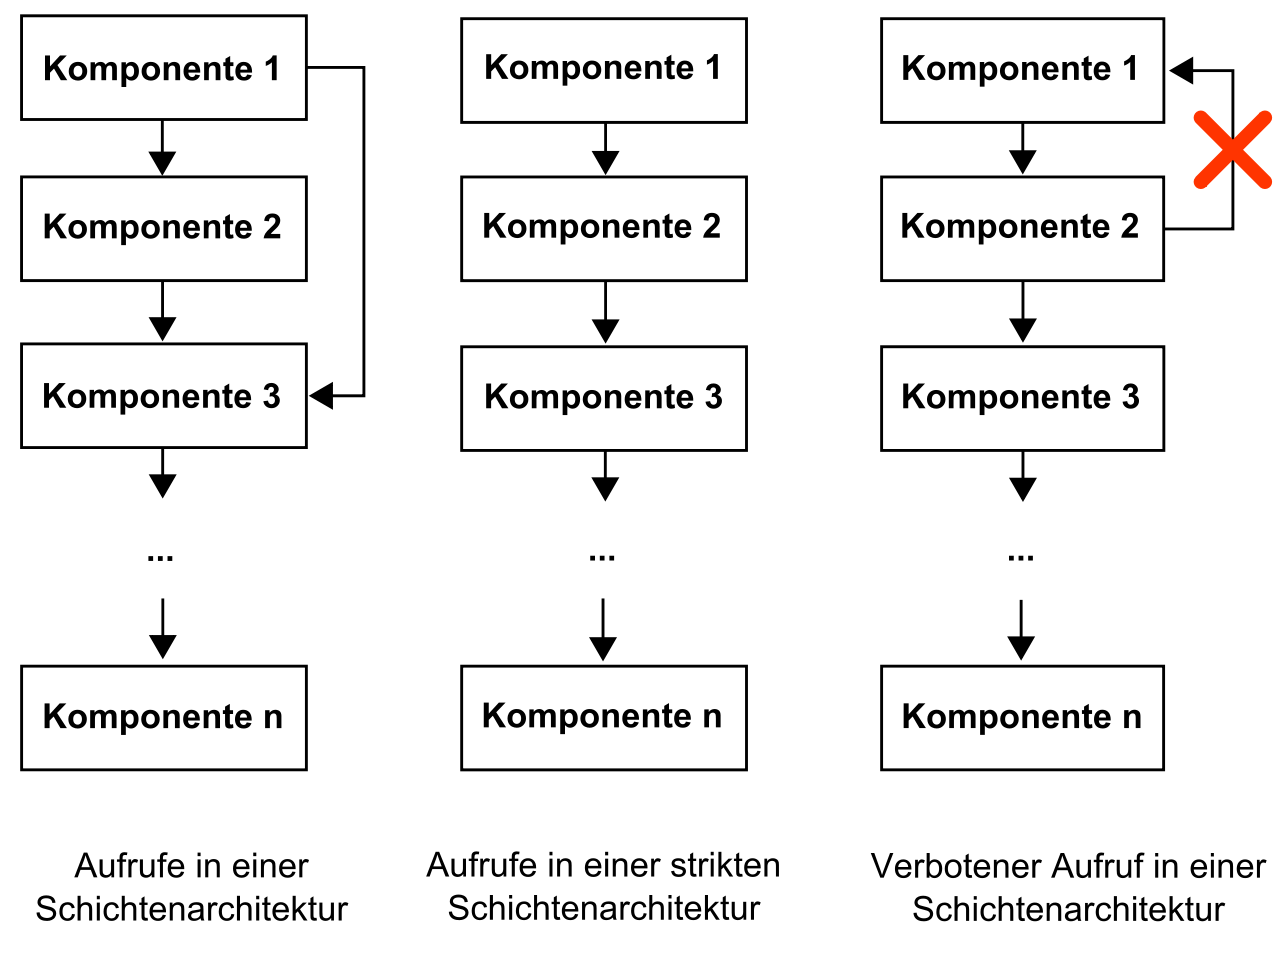
\includegraphics[width=0.3\textwidth]{images/layers}
		\label{fig:layers}
		\caption{Layers}
	\end{center}
\end{figure}

\begin{figure}[h]
	\begin{center}
		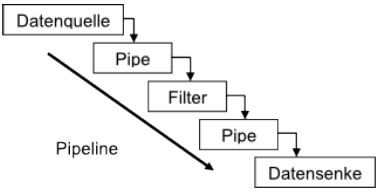
\includegraphics[width=0.3\textwidth]{images/pipes_filters}
		\label{fig:pipes_filters}
		\caption{Pipes and Filters}
	\end{center}
\end{figure}

\begin{figure}[h]
	\begin{center}
		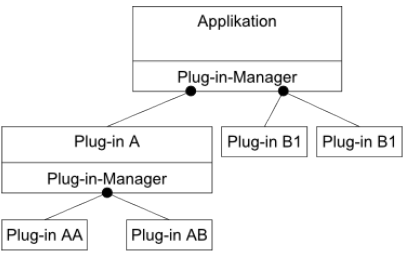
\includegraphics[width=0.3\textwidth]{images/plugin}
		\label{fig:plugin}
		\caption{Plugin}
	\end{center}
\end{figure}

\begin{figure}[h]
	\begin{center}
		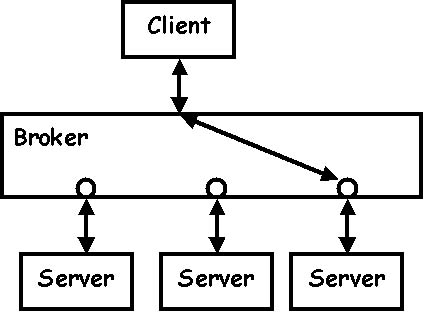
\includegraphics[width=0.3\textwidth]{images/broker}
		\label{fig:broker}
		\caption{Broker}
	\end{center}
\end{figure}

\begin{figure}[h]
	\begin{center}
		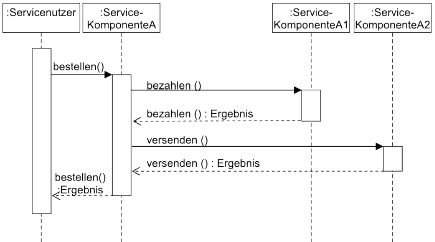
\includegraphics[width=0.3\textwidth]{images/soa}
		\label{fig:soa}
		\caption{SOA}
	\end{center}
\end{figure}

\begin{figure}[h]
	\begin{center}
		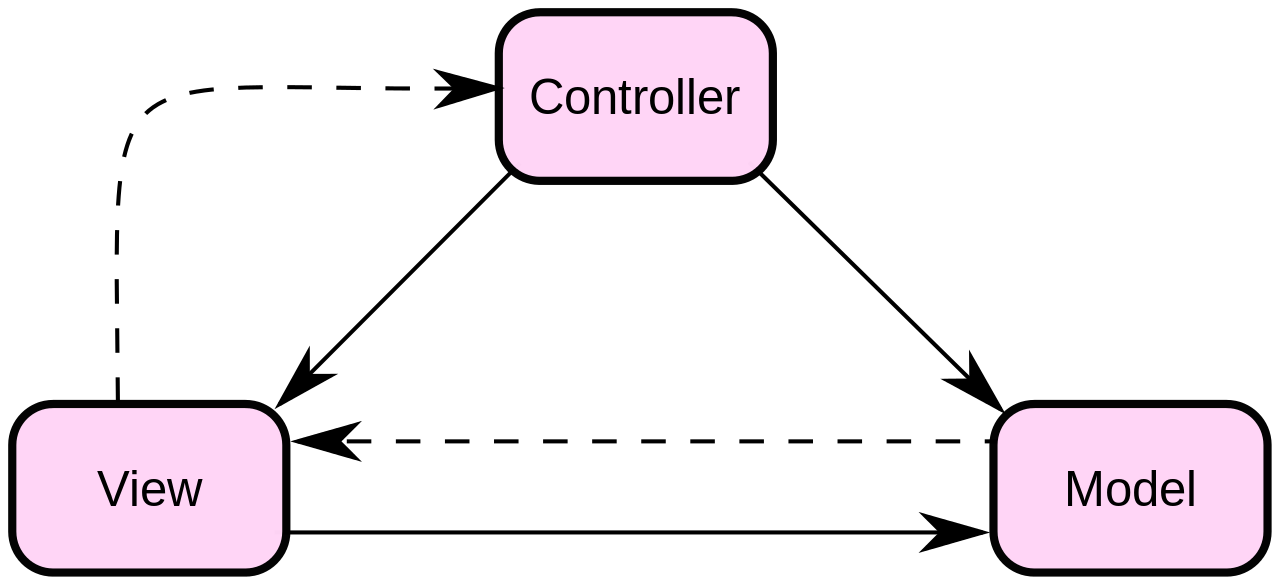
\includegraphics[width=0.3\textwidth]{images/mvc}
		\label{fig:mvc}
		\caption{MVC}
	\end{center}
\end{figure}

\clearpage

\section{Entwurfsmuster}

\begin{figure}[h]
	\begin{center}
		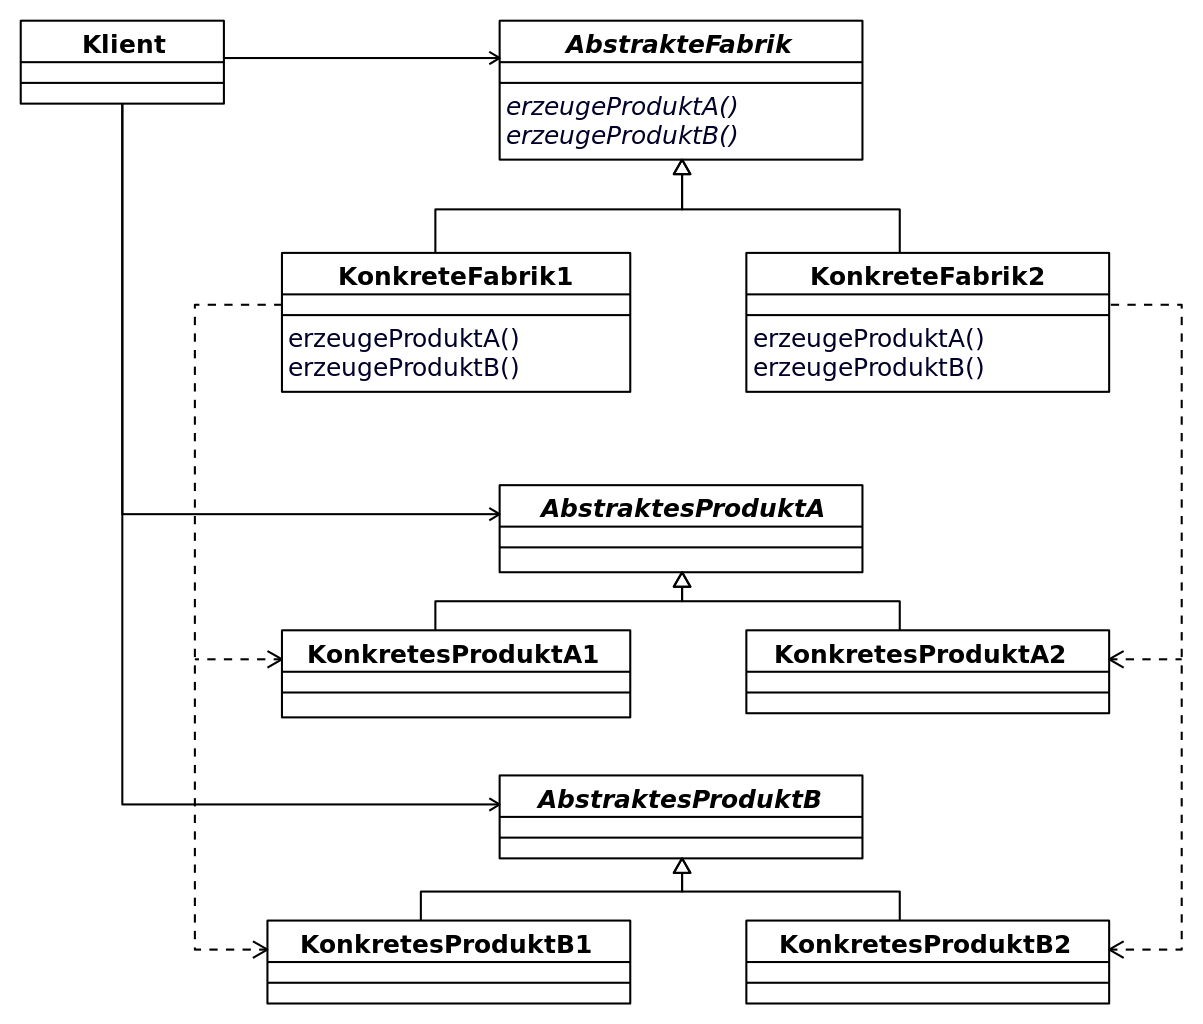
\includegraphics[width=0.3\textwidth]{images/abstract_factory}
		\label{fig:abstract_factory}
		\caption{Abstract Factory}
	\end{center}
\end{figure}

\begin{figure}[h]
	\begin{center}
		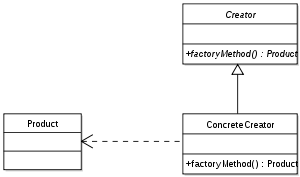
\includegraphics[width=0.3\textwidth]{images/factory}
		\label{fig:factory}
		\caption{Factory}
	\end{center}
\end{figure}

\begin{figure}[h]
	\begin{center}
		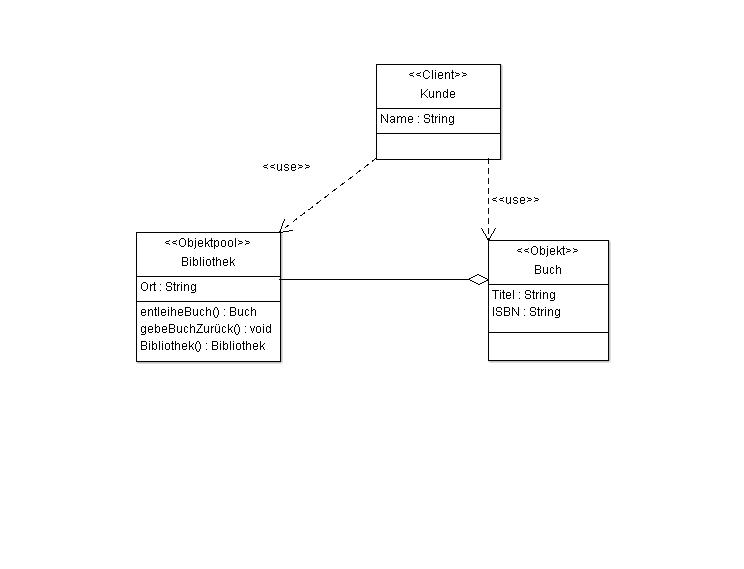
\includegraphics[width=0.3\textwidth]{images/object_pool}
		\label{fig:object_pool}
		\caption{Object Pool}
	\end{center}
\end{figure}

\begin{figure}[h]
	\begin{center}
		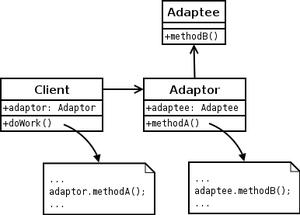
\includegraphics[width=0.3\textwidth]{images/adapter}
		\label{fig:adapter}
		\caption{Adapter}
	\end{center}
\end{figure}

\begin{figure}[h]
	\begin{center}
		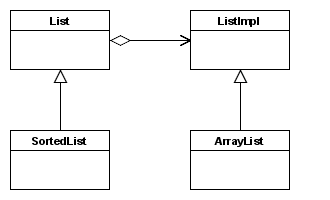
\includegraphics[width=0.3\textwidth]{images/bridge}
		\label{fig:bridge}
		\caption{Bridge}
	\end{center}
\end{figure}

\begin{figure}[h]
	\begin{center}
		
\includegraphics[width=0.3\textwidth]{images/composite}
		\label{fig:composite}
		\caption{Composition}
	\end{center}
\end{figure}

\begin{figure}[h]
	\begin{center}
		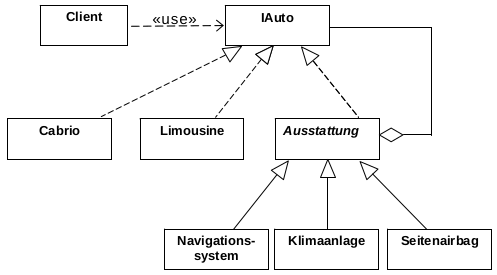
\includegraphics[width=0.3\textwidth]{images/decorator}
		\label{fig:decorator}
		\caption{Decorator}
	\end{center}
\end{figure}

\begin{figure}[h]
	\begin{center}
		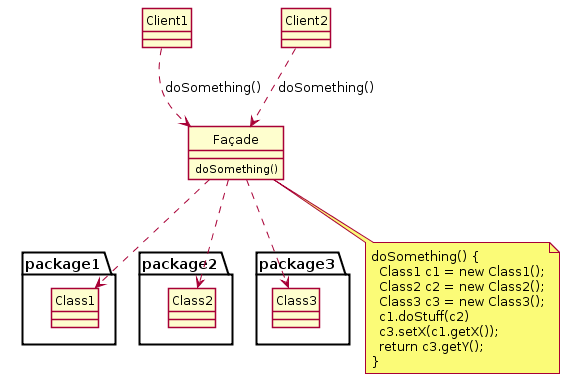
\includegraphics[width=0.3\textwidth]{images/facade}
		\label{fig:facade}
		\caption{Facade}
	\end{center}
\end{figure}

\begin{figure}[h]
	\begin{center}
		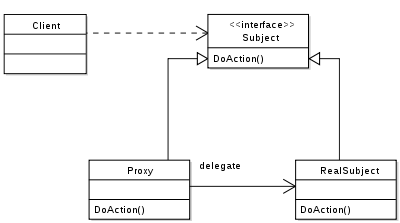
\includegraphics[width=0.3\textwidth]{images/proxy}
		\label{fig:proxy}
		\caption{Proxy}
	\end{center}
\end{figure}

\begin{figure}[h]
	\begin{center}
		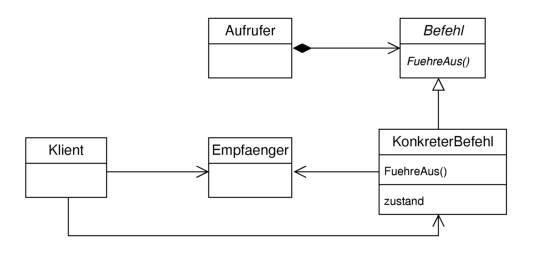
\includegraphics[width=0.3\textwidth]{images/command}
		\label{fig:command}
		\caption{Command}
	\end{center}
\end{figure}

\begin{figure}[h]
	\begin{center}
		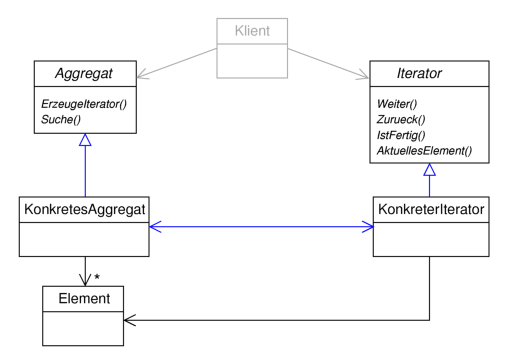
\includegraphics[width=0.3\textwidth]{images/iterator}
		\label{fig:iterator}
		\caption{Iterator}
	\end{center}
\end{figure}

\begin{figure}[h]
	\begin{center}
		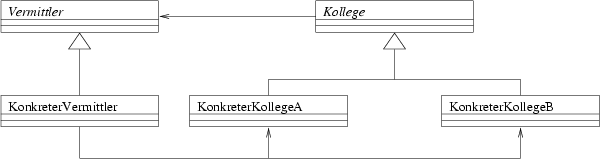
\includegraphics[width=0.3\textwidth]{images/mediator}
		\label{fig:mediator}
		\caption{Mediator}
	\end{center}
\end{figure}

\begin{figure}[h]
	\begin{center}
		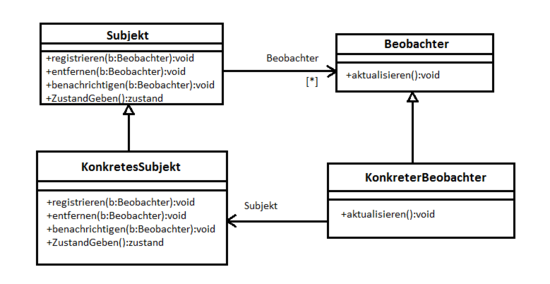
\includegraphics[width=0.3\textwidth]{images/observer}
		\label{fig:observer}
		\caption{Observer}
	\end{center}
\end{figure}

\begin{figure}[h]
	\begin{center}
		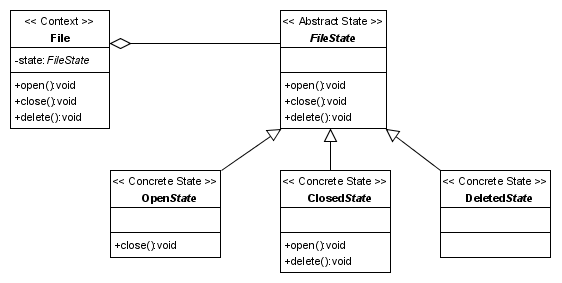
\includegraphics[width=0.3\textwidth]{images/state}
		\label{fig:state}
		\caption{State}
	\end{center}
\end{figure}

\begin{figure}[h]
	\begin{center}
		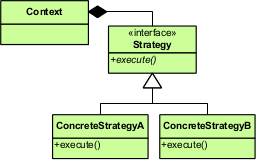
\includegraphics[width=0.3\textwidth]{images/strategy}
		\label{fig:strategy}
		\caption{Strategy}
	\end{center}
\end{figure}

\begin{figure}[h]
	\begin{center}
		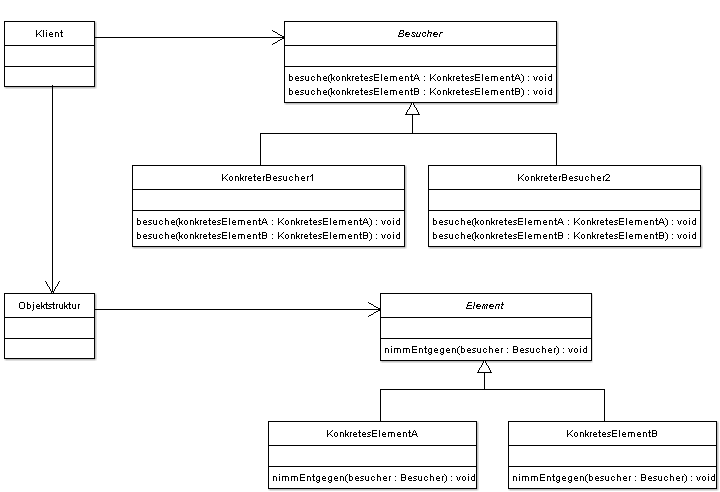
\includegraphics[width=0.3\textwidth]{images/visitor}
		\label{fig:visitor}
		\caption{Visitor}
	\end{center}
\end{figure}

\end{document}


% Hier kommmen Tabellen und Bilder
%\listoftables
%\listoffigures

\end{document}
%% Dokument ENDE %%%%%%%%%%%%%%%%%%%%%%%%%%%%%%%%%%%%%%%%%%%%%%%%%%%%%%%%%%

